\chapter{The CMS experiment}
\label{chap:cms}

\section{Introduction}
With a circumference of 27~km, the Large Hadron Collider (LHC)~\cite{} at CERN is both the largest and most powerful particle accelerator in the world. The machine is designed to collide hadrons together with sufficiently high energy and frequency to enable stringent tests of the SM at the electroweak energy scale. The ATLAS~\cite{}, ALICE~\cite{}, CMS~\cite{} and LHCb~\cite{} experiments are situated at four independent locations along the LHC ring, at which the oppositely circulating hadron beams are focused and brought into collision. Each experiment consists of a particle detector apparatus to measure the products of the hadron collisions, where the design of the detector is chosen to facilitate the respective physics programme: ATLAS and CMS are general purpose detectors designed to measure a wide range of physics processes, whereas LHCb and ALICE are more specialised, focusing on flavour physics and heavy-ion physics respectively. 

The measurements presented in this thesis are performed using data collected by the CMS experiment. This chapter serves as an introduction to both the LHC and the CMS detector, and will help the reader understand how the design of these machines enable the predictions of the SM to be accurately probed using high energy hadron collisions. After introducing the operation and design of the machines in sections \ref{sec:lhc} and \ref{sec:cms}, the focus shifts towards the techniques used to reconstruct the collision products in the CMS detector, detailed in \ref{sec:particle_flow}. Here, particular attention is given to the objects which are most relevant for the \Hgg measurements outlined in chapters~\ref{chap:hgg_overview}--\ref{chap:hgg_results}. Following this, the chapter concludes by looking at a future operation of the LHC machine, known as the High-Luminosity LHC (HL-LHC)~\cite{}, where the rate of collisions will be increased to approximately five times the nominal value. To accommodate this, many parts of the CMS detector will need to be upgraded. Section \ref{sec:hgcal} details one of the key parts of the upgrade programme known as the high granularity calorimeter (HGCAL)~\cite{}. The application of a Boosted Decision Tree (BDT) algorithm to identify electrons and photons from hadronic objects in the HGCAL Level-1 trigger system is detailed. Finally, a simulation-only study is presented in section \ref{sec:trilinar}, looking at the physics reach of the HL-LHC in terms of the sensitivity to the Higgs boson self coupling from top-associated Higgs boson production.

\section{Large Hadron Collider}\label{sec:lhc}

\begin{figure}[htb!]
  \centering
  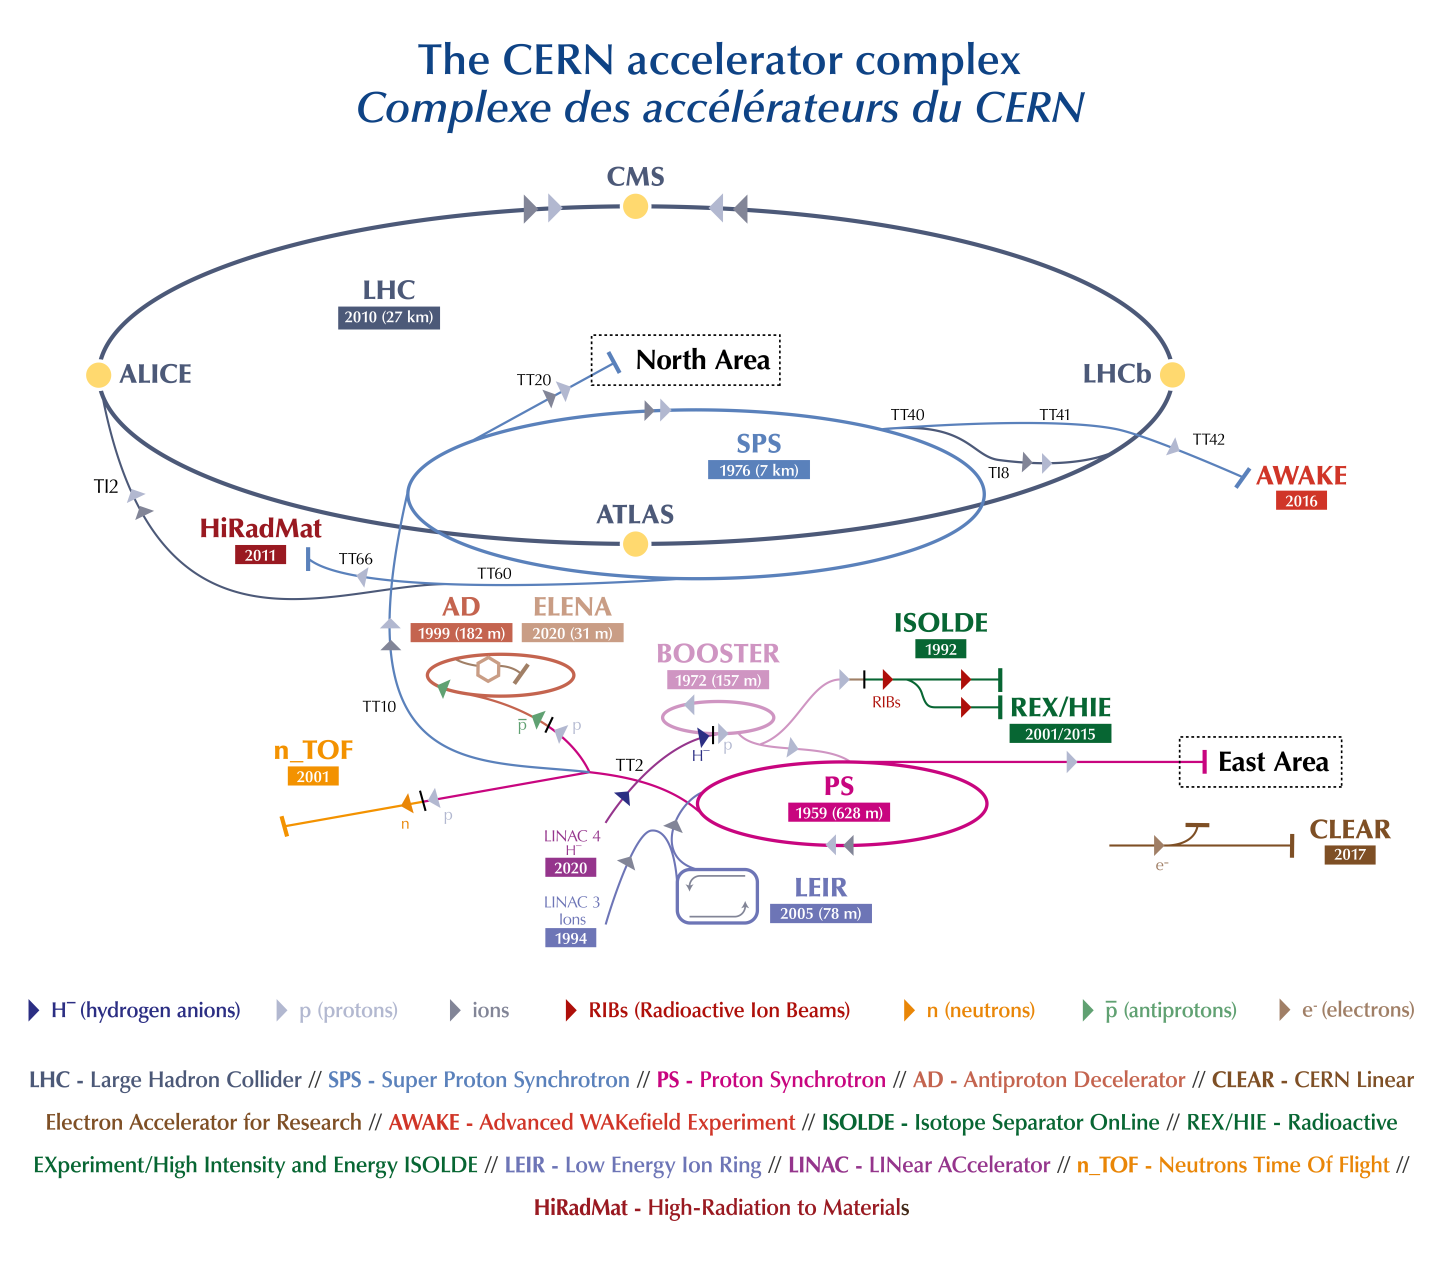
\includegraphics[width=1\textwidth]{Figures/cms/cern_accelerator.png}
  \caption[The CERN accelerator complex]
  {
    An illustration of the CERN accelerator complex, including the four main LHC experiments: ATLAS, ALICE, CMS, and LHCb. The LINAC 2, BOOSTER, PS and SPS are used to sequentially accelerate the proton beams, at which point they are injected into the LHC ring. Diagram is taken from Ref.~\cite{Mobs:2684277}.
  }
  \label{fig:cern_accelerator_complex}
\end{figure}

The LHC is situated 100~m underground the French-Swiss border in the tunnel which previously housed the LEP collider~\cite{}. Both proton-proton (p-p) collisions and heavy ion collisions are performed, where the former is used for measurements at the electroweak scale such as those presented in this thesis. Therefore p-p collisions will be the focus of this section. A chain of machines, known as the CERN accelerator complex, are used to progressively accelerate protons to higher and higher energies, until they are eventually injected into the LHC ring and brought into collision. The full CERN accelerator complex, including the LHC and its experiments are illustrated in Figure \ref{fig:cern_accelerator_complex}.

Firstly, protons are extracted by stripping electrons from hydrogen atoms using a strong electric field. The protons are sequentially accelerated to an energy of 50~MeV by the Linear Accelerator 2 (LINAC 2), to 1.4~GeV in the BOOSTER, and to 25~GeV in the Proton Synchotron (PS). Here, they are additionally spaced into bunches, with each bunch containing several billion protons. Following this, the bunched beams are fed into the Super Proton Synchotron (SPS), accelerated to an energy of 540~GeV and finally injected into the two concentric LHC beam pipes. The beam travels clockwise in the first pipe, and counter-clockwise in the second, producing two counter-circulating proton beams in the LHC ring. This injection is performed until each beam consists of 2808 proton bunches, with a spacing between them of around 25~ns.

A series of 1,232 super-conducting dipole magnets are located along the LHC ring to keep the beams in a circular orbit. These bending magnets are cooled to a temperature of 1.9~K using superfluid helium. Sixteen radiofrequency (RF) cavities are used to accelerate the beams from 540~GeV to the final beam energy. As the beam energy increases, the magnetic field delivered by the bending magnets is increased accordingly to maintain the circular trajectories of the beams. Currently, the highest energy reached for stable operation is 6.5~TeV per beam, which corresponds to a bending magnetic field of 8.3~T. Quadrapole magnets are then used to focus the protons beams at the four interaction points, where the beams are made to collide every 25~ns with a corresponding centre-of-mass energy of $\sqrt{s}=13$~TeV. Note, this is slightly below the maximum LHC design energy of 14~TeV, which would require an energy of 7~TeV per beam; this is expected to be achieved either during run 3 of the LHC (beginning 2022) or during the HL-LHC operation (beginning 2027).

\subsection{Luminosity}
The rate of a particular physics process, $R$, in an LHC experiment is governed by the following relation,

\begin{equation}\label{eq:lumi_rate}
    R = \sigma(\sqrt{s}) \cdot \mathcal{L}_{\rm{inst}}
\end{equation}
\noindent
where $\sigma$ is the cross section of the process of interest, and $\mathcal{L}_{\rm{inst}}$ is the instantaneous luminosity of the LHC machine. The cross section depends on the collision centre-of-mass energy, $\sqrt{s}$, such that raising the collision energy can increase the probability of rare, high-energy processes. The instantaneous luminosity depends solely on the beam parameters according to~\cite{},

\begin{equation}\label{eq:inst_lumi}
    \mathcal{L}_{\rm{inst}} = \frac{n_bN_b^2f_{\rm{rev}}\gamma_r}{4\pi\epsilon_n\beta^*}F,
\end{equation}

\noindent
where $n_b$ is the number of bunches per beam, $N_b$ is the number of particles per bunch, $f_{\rm{rev}}$ is the revolution frequency, $\gamma_r$ is the relativistic gamma factor, $\epsilon_n$ is the normalised transverse beam emittance, $\beta^*$ is the beta-function at the collision point, and $F$ is a reduction factor which accounts for the crossing angle of the beams at the collision point. Ultimately, the exploration of rare events in an LHC experiment requires both high energy and high luminosity.

\begin{figure}[htb!]
  \centering
  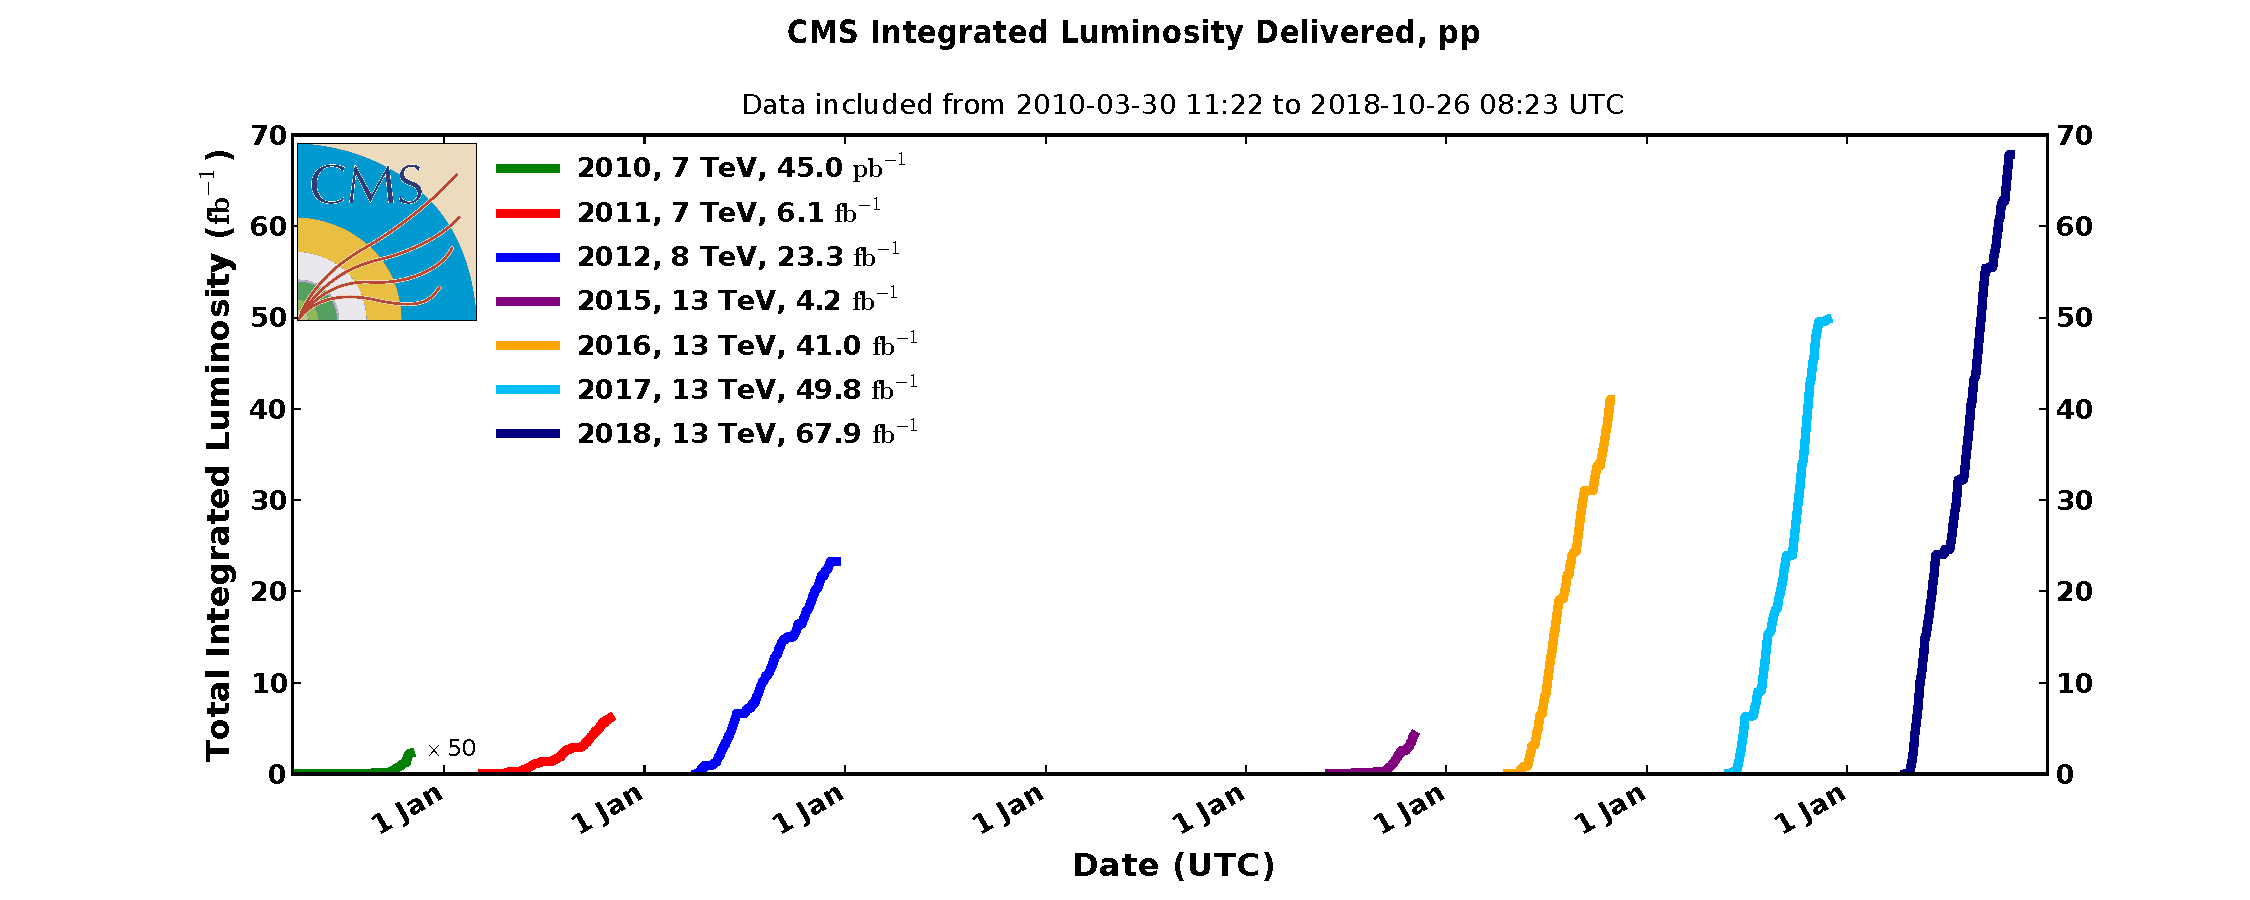
\includegraphics[width=1\textwidth]{Figures/cms/luminosity.pdf}
  \caption[The total integrated luminosity delivered to the CMS experiment]
  {
    The total integrated luminosity delivered to the CMS experiment as a function of time, for each year of operation.
    Figure is taken from Ref.~\cite{CMSLumiPublic}.
  }
  \label{fig:luminosity}
\end{figure}

The LHC was initially designed to run with an instantaneous luminosity of $1\times10^{34}$~cm$^{\rm{2}}$~s$^{\rm{-1}}$. During the 2016-2018 data-taking period this design luminosity was exceeded, eventually levelling at a value of $2 \times 10^{34}$~cm$^{\rm{2}}$~s$^{\rm{-1}}$ for most of the 2018 operation. By integrating the relation in equation \ref{eq:lumi_rate}, we arrive at an expression for the number of events of the process of interest, $N=\sigma\cdot\mathcal{L}$, where $\mathcal{L}$ is the time-\textit{integrated luminosity}, and is a direct measure of the amount of p-p collision data delivered to a collider experiment. Figure~\ref{fig:luminosity} summarises the total integrated luminosity delivered to the CMS experiment throughout its operation. There have been two active phases of the LHC, separated by a shutdown period for upgrades. Run 1 began in 2010 with $\sqrt{s}=7$~TeV, continuing to 2011, such that a total of 6.1~\fbinv of data were collected at this centre-of-mass energy. In 2012, the energy was increased to $\sqrt{s}=8$~TeV, and a further 23.3~\fbinv of data were collected. This Run 1 dataset was the one used for the Higgs boson discovery~\cite{}. 

Run 2 commenced in 2015 and finished in 2018, where protons were collided with $\sqrt{s}=13$~TeV for the full data-taking period. The increase in instantaneous luminosity (gradient of the lines in Figure \ref{fig:luminosity}) during this period has allowed for an extremely large p-p collision dataset to be accumulated, therefore enabling a large improvement in the statistical precision of the measured processes of interest. The results presented in this thesis use data collected during the 2016-2018 data-taking period. In practice, the CMS experiment operates with a data-taking efficiency of around 90\%, such that the amount of data recorded by the experiment and available for physics analysis, over this period, is approximately 137~\fbinv.

One of the drawbacks of increasing the instantaneous luminosity is the enhancement of \textit{pileup}, defined as the number of additional inelastic p-p collisions for each hard-scattering process of interest. As pileup increases, more sophisticated techniques are required to separate the rare process of interest from the objects originating from pileup interactions. In 2016, the mean number of pileup interactions was 23 per bunch crossing, rising to 32 in both the 2017 and 2018 periods. During the HL-LHC phase of operation, the pileup will increase up to a maximum value of around 200, which poses a major challenge to maintain the current excellent reconstruction performance of the CMS detector.

\section{The CMS detector}\label{sec:cms}
CMS is one of two general purpose particle detectors at the LHC~\cite{}, located close to the French village of Cessy. It is over 28~m long, 15~m in diameter, and weighs approximately 14,000~tons. The detector is designed to overcome the experimental challenges that arise in a high-energy collision environment with $\mathcal{O}(1000)$ charged particles being produced every 25~ns. This includes a high level of spatial and timing granularity, with many synchronized detector electronic channels, to maintain a sufficiently low occupancy in these conditions. In addition, the detector and front end electronics must be sufficiently radiation-hard to accommodate the high flux of particles.

One of the main goals of the CMS physics programme was the discovery, and is now the measurement of the Higgs boson and its interactions with other particles. Moreover, the programme includes the precise measurement of other rare processes in the SM, and the search for new BSM physics such as supersymmetry or extra dimensions. To achieve these goals, the detector is designed to:

\begin{itemize}
    \item Identify and reconstruct muons with excellent efficiency and precision. This must be achieved over a wide range of muon energies and angles. In addition, the charge of a muon must be ascertained to a high level of accuracy. The reconstruction of muons is central to Higgs boson measurements, specifically in the \Hfl decay channel.
    \item Achieve a good momentum resolution for charged particles, as well as have the ability to locate secondary vertices consistent with originating from $\tau$'s and b quarks.
    \item Measure the energy of electrons and photons with excellent resolution over a wide geometrical coverage. Additionally, the detector is able to isolate photons and electrons efficiently in a high occupancy environment. These characteristics are key to the \Hgg measurement described in chapters \ref{chap:hgg_overview}-\ref{chap:hgg_results}.
    \item Identify sprays of hadrons, known as jets, which originate from the hadronisation of quarks and gluons, and achieve a good dijet mass resolution.
    \item Accurately calculate the missing energy in an event, which is the key signature of neutrinos or potential BSM particles which do not interact with the detector material.
\end{itemize}

\begin{figure}[htb!]
  \centering
  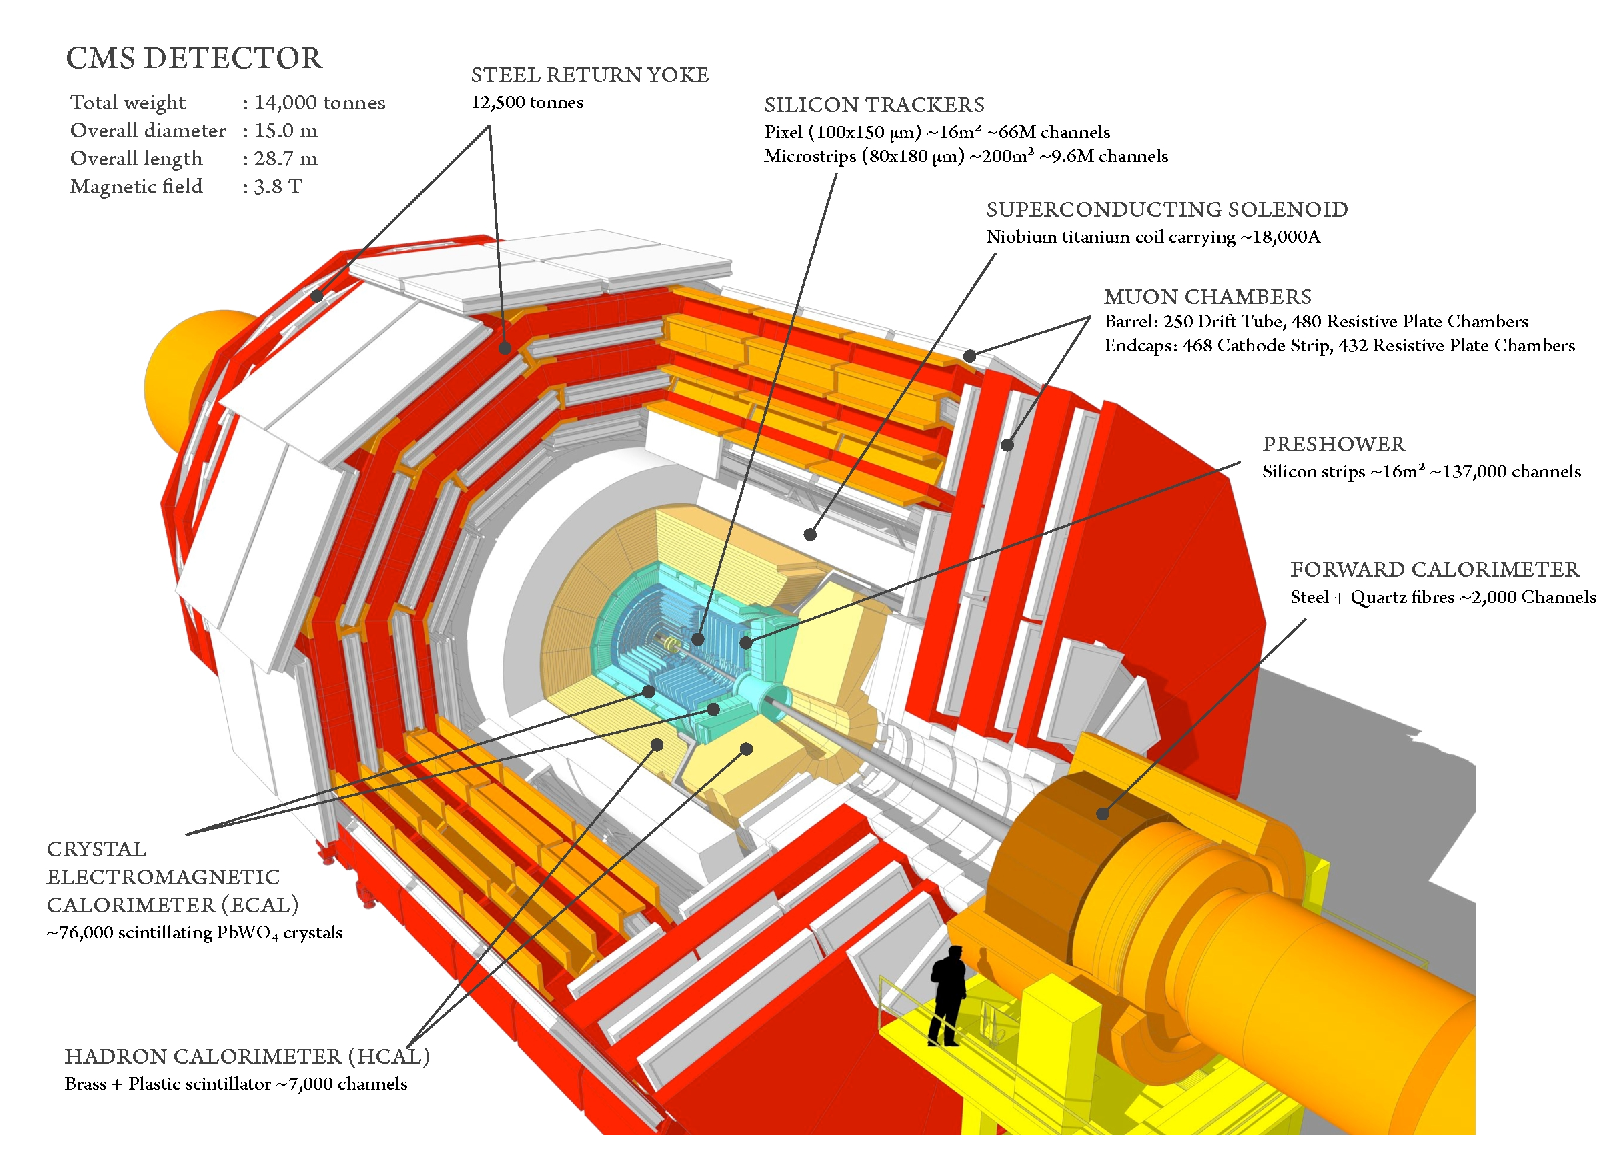
\includegraphics[width=.8\textwidth]{Figures/cms/cms_detector.pdf}
  \caption[The CMS detector]
  {
    A schematic of the CMS detector. Part of the detector has been removed so that the layout is visible. Figure is taken from Ref.~\cite{Sakuma_2014}.
  }
  \label{fig:cms_detector}
\end{figure}

A schematic of the CMS detector is provided in Figure~\ref{fig:cms_detector}. The detector consists of a number of components layered around the beam axis, where each component is comprised of a cylindrical \textit{barrel} section and two \textit{endcaps}. At the heart of this (almost) hermetic cylindrical design is the 3.8~T superconducting solenoid magnet, which provides an extremely high bending power for charged particles traversing the inner region of the detector. Within the coil of the 13~m long, 6~m in diameter solenoid lies the silicon tracker (section \ref{sec:cms_tracker}), the homogeneous crystal electromagnetic calorimeter (section \ref{sec:cms_ecal}), and the sampling hadronic calorimeter (section \ref{sec:cms_hcal}), listed in increasing distance from the interaction point. The muon detection system (section \ref{sec:cms_muon}) is embedded within the iron return yolk of the solenoid. This system of subdetectors, and their respective layering, enables the precise reconstruction of the wide range of physics objects produced in hadron collisions.

\subsection{Co-ordinate system}
A right-handed Cartesian co-ordinate system is adopted, centred at the nominal interaction point, such that the $x$-axis points towards the centre of the LHC ring, the $y$-axis points vertically upwards, and the $z$-axis points in the direction of the counter-clockwise beam. It is more convenient to use a cylindrical co-ordinate system where the direction of an outgoing particle is expressed using the Lorentz-invariant quantities: $\phi$ and $\eta$. Here, $\phi \in [-\pi,\pi]$ is defined as the azimuthal angle in the ($x-y$) plane, relative to the $x$-axis. The quantity $\eta$, referred to as the pseudorapidity, is a measure of the polar angle relative to the beam axis, $\theta$, such that,
\begin{equation}
    \eta = - \ln[\tan(\theta/2)].
\end{equation}
Particles with high values of $\eta$ correspond to a direction close to the LHC beampipe, and are said to be \textit{forward}. The distance measure in the $(\eta,\phi)$ space is defined as $\Delta R = \sqrt{\Delta\eta^2+\Delta\phi^2}$. 

In processes of interest, particles are generally produced with a high momentum in the plane perpendicular to the beam axis. As a result, a useful quantity to characterise a particle is the transverse momentum, $p_T = \sqrt{p_x^2+p_y^2}$, defined as the projection of the particle's total momentum onto this transverse plane. Finally, the missing transverse momentum, \met, is defined as the magnitude of the negative vector sum of particle's momenta in the transverse plane.

\subsection{Tracker}\label{sec:cms_tracker}
The tracker is the innermost component of the CMS detector~\cite{}, and is designed to measure the trajectory of charged particles deflected by the 3.8~T magnetic field. The tracker is also able to accurately locate the position of the primary hard scattering interaction vertex, as well as identify secondary interaction vertices which originate from the decay of $\tau$'s or b quarks.

\begin{figure}[htb!]
  \centering
  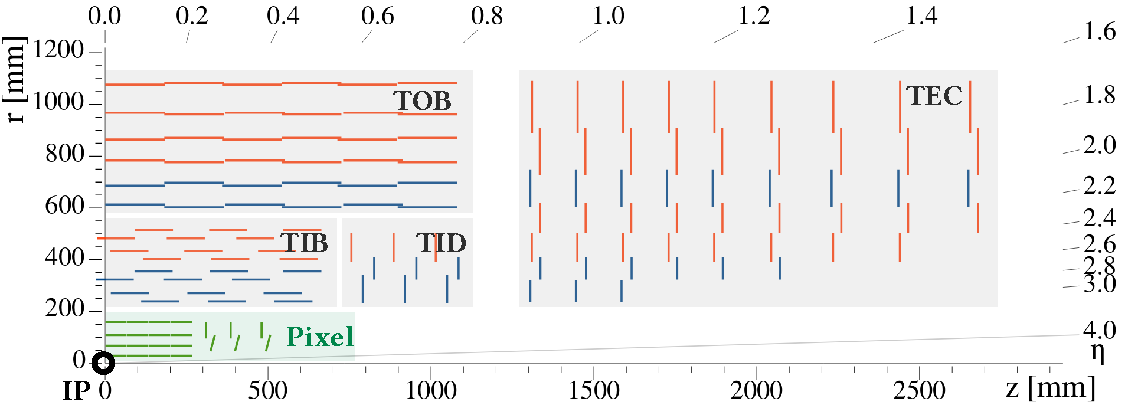
\includegraphics[width=.8\textwidth]{Figures/cms/tracker.pdf}
  \caption[The CMS silicon tracker]
  {
    A diagram showing one quarter of the CMS tracker in the $r$-$z$ view, where $r$ is a measure of the radial distance in the ($x$-$y$)-plane. The pixel detector, closest to the interaction point (IP, black circle) is shown in green. The sections of the silicon strip tracker (TIB, TID, TOB, TEC) are also shown, where the red and blue lines signify one-sided and two-sided strips respectively. Figure has been adapted from the original in Ref.~\cite{CERN-LHCC-2017-009}.
  }
  \label{fig:cms_tracker}
\end{figure}

\begin{itemize}
    \item Design requirements, 25ns, radiation hard, material budget etc.
    \item Layout: $\eta$ coverage. Pixel, strip. Spatial and temporal Resolutions. Number of hits
    \item How to infer the momentum from trajectory, worsens as momentum increases. Performance. Vertex performance. Matrial.
    \item Upgrade to the pixel detector.
\end{itemize}


\subsection{Electromagnetic calorimeter}\label{sec:cms_ecal}
Meausre energy of electromagnetic showers from photons and electrons.

\begin{itemize}
    \item Energy resolution plot
\end{itemize}

\subsection{Hadronic calorimeter}\label{sec:cms_hcal}
Measure energy of sprays of hadrons, known as jets, originating from the hadronisation of the quarks and gluons.

\subsection{Muon chambers}\label{sec:cms_muon}

\subsection{Trigger}\label{sec:trigger}
Maintain signal efficiency whilst minimising the rate. L1T coarser objects as limited time. Online reconstruction. 

\subsection{Summary}
Add classic different object cross section diagram. Lead into reconstruction.

\section{Object reconstruction: particle flow}\label{sec:particle_flow}
Holistic.
Offline reconstruction. Combines information from CMS subdetectors. Focus on Supercluster reconstruction for photons.

\section{Monte Carlo generators}\label{sec:mc}
Integral is intractable... use simulation. PDFs etc. Parton shower.

\section{The High-Luminosity LHC}
\subsection{Introduction}
Refer to equation \ref{eq:inst_lumi}

\subsection{The High Granularity Calorimeter}
\begin{itemize}
    \item Explain BDT: a bit about training machine learning algorithms (page). Also DNN
    \item Show $e\gamma$-ID 
\end{itemize}

\subsection{Physics reach of the HL-LHC}\label{sec:trilinar}
\begin{itemize}
    \item Trilinear stuff
\end{itemize}